\section{Products \label{sect:products}}

The products of DM are not the data products defined in \citeds{LSE-163},
but rather the artifacts, systems, and services which will be used by the
operational LSST system to generate those data products.

In \secref{sect:dmarc}, we briefly described the high level approach being taken to the design of the DM products, while \appref{sect:prodlist} provides a complete list of products, including the technical manager, WBS element, and product owner for each.
That information is summarized in the product tree shown in \figref{fig:prods}.

Each DM product is being developed to satisfy one or more of the requirements placed upon the DM subsystem. \citeds{LDM-148} provides a tracing from each product to and from the relevant requirements.
These requirements are drawn from \citeds{LSE-61}, the DM System Requirements document.
The requirements \citeds{LSE-61} are themselves traced to higher level requirements in
the Observatory System Specifications (OSS; \citeds{LSE-30}) (See also \figref{fig:doctree}).
\appref{sect:tracefor} traces DM requirements to higher level requirements, and \appref{sect:traceback} traces relevant higher-level requirements to DM.

\begin{figure}[htbp]
	\begin{center}
		 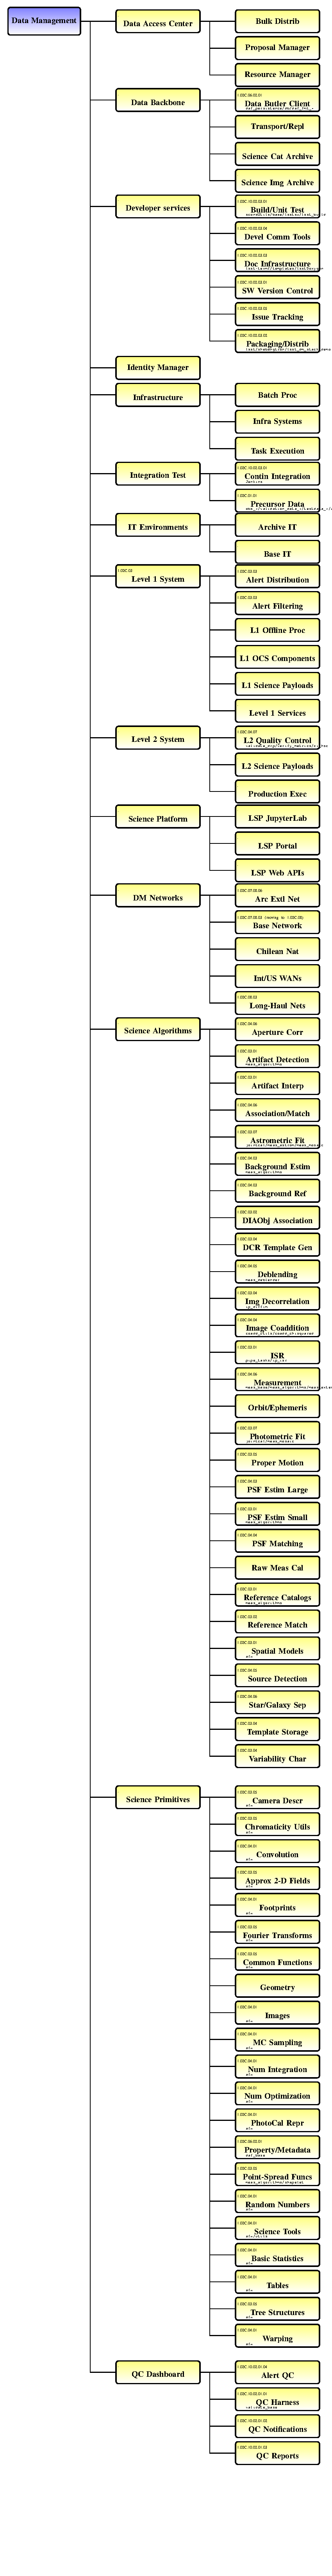
\includegraphics[height=19cm]{ProductTree}
         \caption{An overview of the DM product tree. This provides just a summary of the highest level items: refer to \appref{sect:prodlist} for the full list.}
         \label{fig:prods}
	 \end{center}
 \end{figure}

Every code repository used by DM must be associated with a product, and hence will have an associated technical manager and product owner.
